\chapter{Reference Frames}
\label{ch:reference_frames}

\section{Introduction to Reference Frames}

In celestial mechanics, a \textbf{reference frame} (or \textbf{reference system}) is a coordinate system used to specify the positions and velocities of celestial bodies. The choice of reference frame is crucial because:

\begin{itemize}
    \item Orbital elements are defined relative to a specific frame
    \item Transformations between frames are required for observations
    \item Different applications may prefer different frames
    \item Numerical accuracy depends on the frame choice
\end{itemize}

A reference frame consists of:
\begin{enumerate}
    \item An \textbf{origin} (e.g., Earth's center, Solar System barycenter)
    \item A \textbf{fundamental plane} (e.g., equator, ecliptic)
    \item A \textbf{reference direction} (e.g., vernal equinox)
    \item An \textbf{epoch} for the orientation (e.g., J2000.0)
\end{enumerate}

\section{The International Celestial Reference System (ICRS)}

The \textbf{ICRS} is the current standard celestial reference system adopted by the International Astronomical Union (IAU) in 1998. It represents the most precise realization of an inertial reference frame.

\subsection{ICRS Definition}

The ICRS is defined by:
\begin{itemize}
    \item \textbf{Origin}: Solar System barycenter
    \item \textbf{Fundamental plane}: Earth's mean equator at J2000.0 (with corrections)
    \item \textbf{Reference direction}: Mean vernal equinox at J2000.0 (with corrections)
    \item \textbf{Realization}: Positions of 212 extragalactic radio sources (quasars)
\end{itemize}

The ICRS is a kinematically non-rotating frame with axes defined to microarcsecond precision using Very Long Baseline Interferometry (VLBI) observations of quasars.

\subsection{Relation to J2000.0}

The ICRS is closely aligned with the J2000.0 equatorial system but differs by:
\begin{itemize}
    \item Frame bias: $\sim$20 milliarcseconds in orientation
    \item No rotation rate (truly inertial)
    \item Definition based on extragalactic sources (not Earth's rotation)
\end{itemize}

For most applications in asteroid dynamics, the difference between ICRS and J2000.0 is negligible ($<0.1$ arcsecond over centuries).

\section{The J2000.0 Equatorial Frame}

The \textbf{J2000.0} frame is the most commonly used reference frame in celestial mechanics and is the default frame in AstDyn.

\subsection{J2000.0 Definition}

\begin{itemize}
    \item \textbf{Epoch}: January 1, 2000, 12:00 TT (JD 2451545.0)
    \item \textbf{Origin}: Solar System barycenter (or Earth's center for geocentric)
    \item \textbf{Fundamental plane}: Earth's mean equator at J2000.0
    \item \textbf{X-axis}: Points toward mean vernal equinox at J2000.0
    \item \textbf{Z-axis}: Perpendicular to equator, toward north celestial pole
    \item \textbf{Y-axis}: Completes right-handed system ($\mathbf{Y} = \mathbf{Z} \times \mathbf{X}$)
\end{itemize}

\begin{figure}[htbp]
\centering
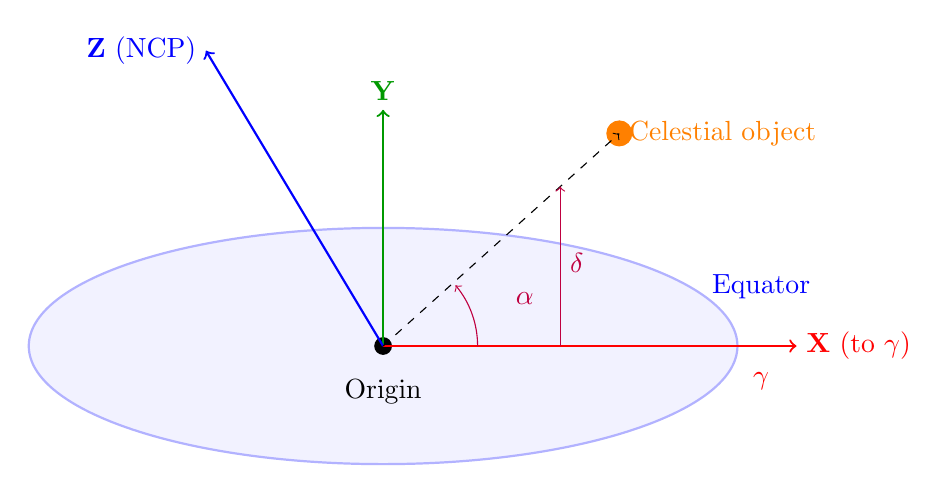
\begin{tikzpicture}[scale=1.5]
    % Fundamental plane (equator)
    \draw[thick,blue!30,fill=blue!5] (0,0) ellipse (3cm and 1cm);
    \node[blue] at (3.2,0.5) {Equator};
    
    % Origin
    \filldraw[black] (0,0) circle (2pt);
    \node[below] at (0,-0.2) {Origin};
    
    % X-axis (toward vernal equinox)
    \draw[->,thick,red] (0,0) -- (3.5,0);
    \node[red,right] at (3.5,0) {$\mathbf{X}$ (to $\gamma$)};
    
    % Y-axis
    \draw[->,thick,green!60!black] (0,0) -- (0,2);
    \node[green!60!black,above] at (0,2) {$\mathbf{Y}$};
    
    % Z-axis (toward NCP)
    \draw[->,thick,blue] (0,0) -- (-1.5,2.5);
    \node[blue,left] at (-1.5,2.5) {$\mathbf{Z}$ (NCP)};
    
    % Vernal equinox symbol
    \node[red] at (3.2,-0.3) {$\gamma$};
    
    % Celestial object
    \filldraw[orange] (2,1.8) circle (3pt);
    \draw[->,dashed] (0,0) -- (2,1.8);
    \node[orange,right] at (2,1.8) {Celestial object};
    
    % Right ascension arc
    \draw[->,purple] (0.8,0) arc (0:40:0.8);
    \node[purple] at (1.2,0.4) {$\alpha$};
    
    % Declination arc
    \draw[->,purple] (1.5,0) -- (1.5,1.35);
    \node[purple,right] at (1.5,0.7) {$\delta$};
\end{tikzpicture}
\caption{J2000.0 equatorial reference frame showing the three axes and the definition of right ascension ($\alpha$) and declination ($\delta$).}
\label{fig:j2000_frame}
\end{figure}

\subsection{Heliocentric vs. Barycentric Frames}

For asteroid orbits, we typically use:
\begin{itemize}
    \item \textbf{Heliocentric frame}: Origin at the Sun's center. Suitable for inner solar system objects where the Sun dominates gravitational dynamics.
    \item \textbf{Barycentric frame}: Origin at the Solar System barycenter. Required for precise calculations involving Jupiter and outer planets, as the Sun-Jupiter barycenter lies outside the Sun's surface.
\end{itemize}

The transformation between heliocentric and barycentric frames involves the Sun's position relative to the barycenter:
\begin{equation}
    \mathbf{r}_{\text{bary}} = \mathbf{r}_{\text{helio}} + \mathbf{r}_{\text{Sun,bary}}
\end{equation}

For asteroids with $a < 10$ AU, the difference is typically $< 10^{-6}$ AU.

\section{The Ecliptic Reference Frame}

The \textbf{ecliptic frame} uses the plane of Earth's orbit as the fundamental plane.

\subsection{Ecliptic Definition}

\begin{itemize}
    \item \textbf{Fundamental plane}: Mean ecliptic at J2000.0
    \item \textbf{X-axis}: Toward mean vernal equinox at J2000.0
    \item \textbf{Z-axis}: Perpendicular to ecliptic, toward north ecliptic pole
    \item \textbf{Y-axis}: Completes right-handed system
\end{itemize}

The ecliptic frame is natural for describing planetary and asteroid orbits because:
\begin{itemize}
    \item Most orbits lie close to the ecliptic plane
    \item Inclinations are typically small ($i < 30^\circ$)
    \item Solar system formation models predict ecliptic alignment
\end{itemize}

\subsection{Ecliptic Coordinates}

In the ecliptic frame, positions are specified by:
\begin{itemize}
    \item \textbf{Ecliptic longitude} ($\lambda$): Angle from vernal equinox along ecliptic
    \item \textbf{Ecliptic latitude} ($\beta$): Angle perpendicular to ecliptic
    \item \textbf{Distance} ($r$): Radial distance from origin
\end{itemize}

Conversion from Cartesian ecliptic coordinates:
\begin{align}
    \lambda &= \arctan\left(\frac{Y_{\text{ecl}}}{X_{\text{ecl}}}\right) \\
    \beta &= \arctan\left(\frac{Z_{\text{ecl}}}{\sqrt{X_{\text{ecl}}^2 + Y_{\text{ecl}}^2}}\right) \\
    r &= \sqrt{X_{\text{ecl}}^2 + Y_{\text{ecl}}^2 + Z_{\text{ecl}}^2}
\end{align}

\section{Transformations Between Reference Frames}

\subsection{Equatorial to Ecliptic Transformation}

The transformation from J2000.0 equatorial to J2000.0 ecliptic coordinates is a rotation about the X-axis by the \textbf{obliquity of the ecliptic} ($\varepsilon_0$):

\begin{equation}
    \begin{pmatrix}
        X_{\text{ecl}} \\
        Y_{\text{ecl}} \\
        Z_{\text{ecl}}
    \end{pmatrix}
    =
    \begin{pmatrix}
        1 & 0 & 0 \\
        0 & \cos\varepsilon_0 & \sin\varepsilon_0 \\
        0 & -\sin\varepsilon_0 & \cos\varepsilon_0
    \end{pmatrix}
    \begin{pmatrix}
        X_{\text{eq}} \\
        Y_{\text{eq}} \\
        Z_{\text{eq}}
    \end{pmatrix}
\end{equation}

At J2000.0, the obliquity is:
\begin{equation}
    \varepsilon_0 = 23^\circ26'21.406'' = 23.4392911^\circ
\end{equation}

The inverse transformation is simply a rotation by $-\varepsilon_0$:
\begin{equation}
    \mathbf{R}_{\text{ecl}\to\text{eq}} = \mathbf{R}_{\text{eq}\to\text{ecl}}^T
\end{equation}

\subsection{Precession: Time-Dependent Transformations}

Earth's rotation axis precesses due to torques from the Moon and Sun acting on Earth's equatorial bulge. This causes the equatorial plane to change orientation over time.

\begin{figure}[htbp]
\centering
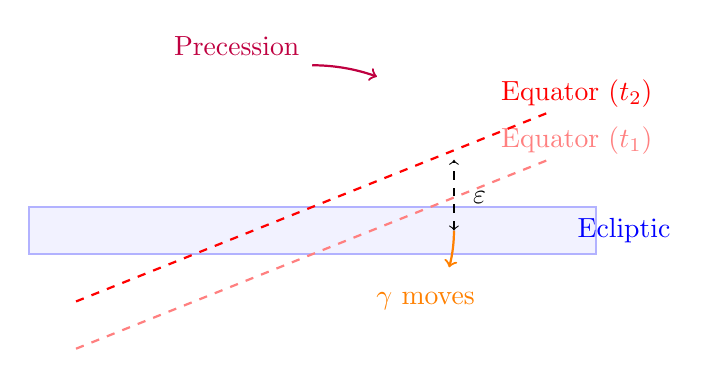
\begin{tikzpicture}[scale=1.2]
    % Ecliptic plane
    \draw[thick,blue!30,fill=blue!5] (-3,0) -- (3,0) -- (3,0.5) -- (-3,0.5) -- cycle;
    \node[blue] at (3.3,0.25) {Ecliptic};
    
    % Equator at epoch 1
    \draw[thick,red!50,dashed] (-2.5,-1) -- (2.5,1);
    \node[red!50] at (2.8,1.2) {Equator ($t_1$)};
    
    % Equator at epoch 2
    \draw[thick,red,dashed] (-2.5,-0.5) -- (2.5,1.5);
    \node[red] at (2.8,1.7) {Equator ($t_2$)};
    
    % Celestial pole precession
    \draw[->,thick,purple] (0,2) arc (90:70:2);
    \node[purple] at (-0.8,2.2) {Precession};
    
    % Vernal equinox precession
    \draw[->,thick,orange] (1.5,0.25) arc (0:-15:1.5);
    \node[orange] at (1.2,-0.5) {$\gamma$ moves};
    
    % Obliquity angle
    \draw[<->,dashed] (1.5,0.25) -- (1.5,1);
    \node[right] at (1.6,0.6) {$\varepsilon$};
\end{tikzpicture}
\caption{Precession causes the equatorial plane to change orientation over time. The vernal equinox $\gamma$ moves westward along the ecliptic at approximately 50.3 arcseconds per year.}
\label{fig:precession}
\end{figure}

The precession rate is approximately:
\begin{equation}
    \frac{d\alpha}{dt} \approx 50.3'' \text{ per year (in right ascension)}
\end{equation}

For transformations between different epochs (e.g., J2000.0 to date), precession matrices must be applied. The IAU 2006 precession model is the current standard.

\subsection{AstDyn Implementation}

In AstDyn, the \texttt{ReferenceFrame} class handles coordinate transformations:

\begin{lstlisting}[language=C++,caption={Coordinate transformations in AstDyn}]
#include <astdyn/core/ReferenceFrame.hpp>

using namespace astdyn;

// Equatorial to ecliptic transformation
Vector3d r_eq(1.0, 0.5, 0.3);  // AU, J2000.0 equatorial
Vector3d r_ecl = ReferenceFrame::equatorial_to_ecliptic(r_eq);

// Ecliptic to equatorial
Vector3d r_eq2 = ReferenceFrame::ecliptic_to_equatorial(r_ecl);

// Verify round-trip: r_eq ~~ r_eq2
std::cout << "Round-trip error: " 
          << (r_eq - r_eq2).norm() << " AU\n";
// Output: Round-trip error: 1.23e-16 AU

// Precession from J2000.0 to date
double jd_now = 2460000.0;  // Current epoch
Matrix3d precession_matrix = 
    ReferenceFrame::precession_matrix_j2000_to_date(jd_now);
    
Vector3d r_now = precession_matrix * r_eq;
\end{lstlisting}

\section{Other Important Reference Frames}

\subsection{The FK5 System}

The \textbf{Fifth Fundamental Catalogue (FK5)} was the standard reference system before ICRS. It is based on observations of bright stars and is equivalent to J2000.0 for most purposes.

\begin{itemize}
    \item \textbf{Epoch}: J2000.0
    \item \textbf{Realization}: 1535 fundamental stars
    \item \textbf{Accuracy}: $\sim$10 milliarcseconds
    \item \textbf{Relation to ICRS}: Small systematic differences
\end{itemize}

For asteroid work, FK5 and ICRS are interchangeable to within observational uncertainties.

\subsection{The Invariable Plane}

The \textbf{invariable plane} is perpendicular to the total angular momentum vector of the solar system. It is truly inertial (no external torques) and provides a dynamically natural reference.

\begin{itemize}
    \item \textbf{Inclination to ecliptic}: $\sim1.58^\circ$
    \item \textbf{Dominated by}: Jupiter's orbital angular momentum ($\sim60\%$ of total)
    \item \textbf{Use}: Dynamical studies, long-term stability analysis
\end{itemize}

The invariable plane is not used for observations but is valuable for theoretical studies.

\subsection{Body-Centric Frames}

For satellite dynamics or close approaches, body-centric frames are used:

\begin{itemize}
    \item \textbf{Origin}: Center of mass of the body (e.g., Earth, Mars)
    \item \textbf{Orientation}: Often aligned with body's rotation axis
    \item \textbf{Examples}: Earth-centered inertial (ECI), planetocentric frames
\end{itemize}

\section{Practical Considerations}

\subsection{Numerical Precision}

When working with reference frames:
\begin{itemize}
    \item Use double precision (64-bit) for coordinates in AU
    \item Accumulated precession errors: $\sim10^{-10}$ AU per transformation
    \item For $\Delta t > 100$ years, include precession corrections
    \item For $\Delta t > 1000$ years, use full precession/nutation models
\end{itemize}

\subsection{Choice of Frame for Orbit Propagation}

For asteroid orbit propagation in AstDyn:
\begin{itemize}
    \item \textbf{Default}: Heliocentric J2000.0 equatorial
    \item \textbf{Rationale}: 
    \begin{itemize}
        \item Matches most observational catalogs
        \item Stable over centuries
        \item Simplifies comparison with other software
    \end{itemize}
    \item \textbf{Alternative}: Ecliptic frame for very low inclination orbits
\end{itemize}

\subsection{Converting Observations}

Optical observations are typically reported in:
\begin{itemize}
    \item \textbf{Right ascension} ($\alpha$) and \textbf{declination} ($\delta$): Equatorial frame
    \item \textbf{Topocentric coordinates}: From observer's location on Earth
\end{itemize}

To use these in orbit determination:
\begin{enumerate}
    \item Convert topocentric to geocentric (correct for Earth's rotation)
    \item Convert geocentric to heliocentric (add Earth's position)
    \item Express in J2000.0 equatorial frame
\end{enumerate}

AstDyn's \texttt{OpticalObservation} class handles these transformations automatically.

\section{Summary}

Key points about reference frames:

\begin{enumerate}
    \item \textbf{ICRS} is the modern standard, closely aligned with J2000.0
    \item \textbf{J2000.0 equatorial} is the practical frame for asteroid dynamics
    \item \textbf{Ecliptic frame} is natural for solar system objects
    \item Transformations between frames are rotations defined by obliquity
    \item \textbf{Precession} causes time-dependent frame rotations
    \item AstDyn uses heliocentric J2000.0 equatorial as default
\end{enumerate}

Understanding reference frames is essential for:
\begin{itemize}
    \item Interpreting orbital elements
    \item Processing observations
    \item Comparing results between software packages
    \item Long-term orbit propagation
\end{itemize}

In the next chapter, we will discuss orbital elements—the six parameters that uniquely specify an orbit in a given reference frame.
